%
% singularities.tex -- 
%
% (c) 2019 Prof Dr Andreas Mueller
%
\section{Development of singularities}
The solution of a partial differential equation depends crucially
on the geometry of the characteristics.
If the projections onto the $x$-$y$-plane of two characteristics 
meet, the solution can no longer be unique.
The solution is only unique if characteristics don't intersect.
Otherwise singularities will develop.

As an example we consider the nonlinear equation of Burgers
\begin{equation}
\frac{\partial u}{\partial t}+u\frac{\partial u}{\partial x}=0.
\label{wellenichtlinear}
\end{equation}
with initial conditions
\[
u(0,x_0)=g(x_0)=e^{-4(x_0-\frac12)^2}.
\]
According to the method of characteristics, we need solution curves for the
vector field
\[
\begin{pmatrix}
1\\
u\\
0
\end{pmatrix}
\]
through the point
$(0,x_0, z_0)$,
i.~e. a solution onf the system of differential equations
\[
\left.
\begin{aligned}
\frac{d}{d\tau} t(\tau)&=1\\
\frac{d}{d\tau} x(\tau)&=z(\tau)\\
\frac{d}{d\tau} z(\tau)&=0
\end{aligned}
\quad
\right\}
\qquad
\Rightarrow
\qquad
\left\{
\quad
\begin{aligned}
t(\tau)&=\tau\\
z(\tau)&=z(0)\\
x(\tau)&=z(0)\tau +x(0)
\end{aligned}
\right.
\]
We read off that the parameter $\tau$ 
is identical to $t$.
The solution surface thus has the parametrization
\[
(t,x_0)\mapsto
\begin{pmatrix}
t\\
g(x_0)t+x_0\\
g(x_0)
\end{pmatrix}.
\]
Projections of characteristics into the $x$-$t$-plane are straight
lines with slope depending on $g(x_0)$.
The larger $g(x_0)$, the more the integral curve veers off to the right.
Large values of the initial condition will thus overtake the smaller
values, creating jump singularities.

At tiem t$t$, the solution has parametrization
\[
x_0\mapsto (g(x_0)t+x_0,g(x_0)).
\]
The graphs in figure~\ref{g} show how the solution develops over time.
It becomes obvious that for sufficiently large time $t$ the solution
surface can not longer be the graph of a function $u(t,x)$.

\begin{figure}
\begin{center}
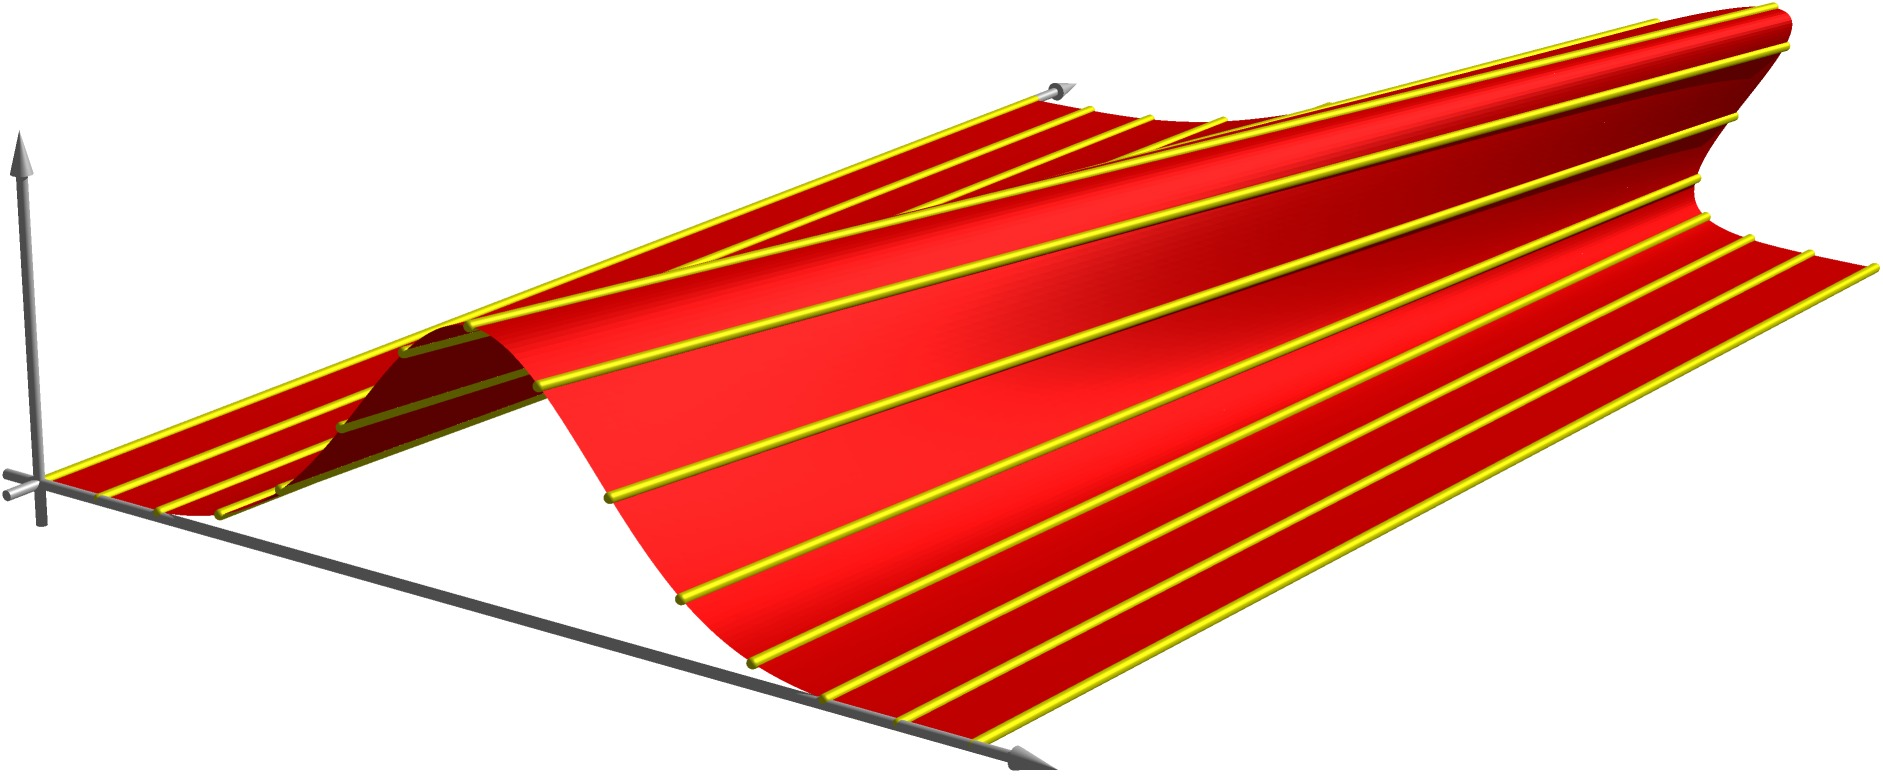
\includegraphics[width=\hsize]{../common/graphics/welle.jpg}
\end{center}
\caption{Solution of the partial differential equation
\eqref{wellenichtlinear} developing a singularity \label{g}}
\end{figure}

